% Dataset and missing-value audit
\section{Dataset and Features}

\begin{frame}{Dataset and Missing-Value Audit}
  \centering
  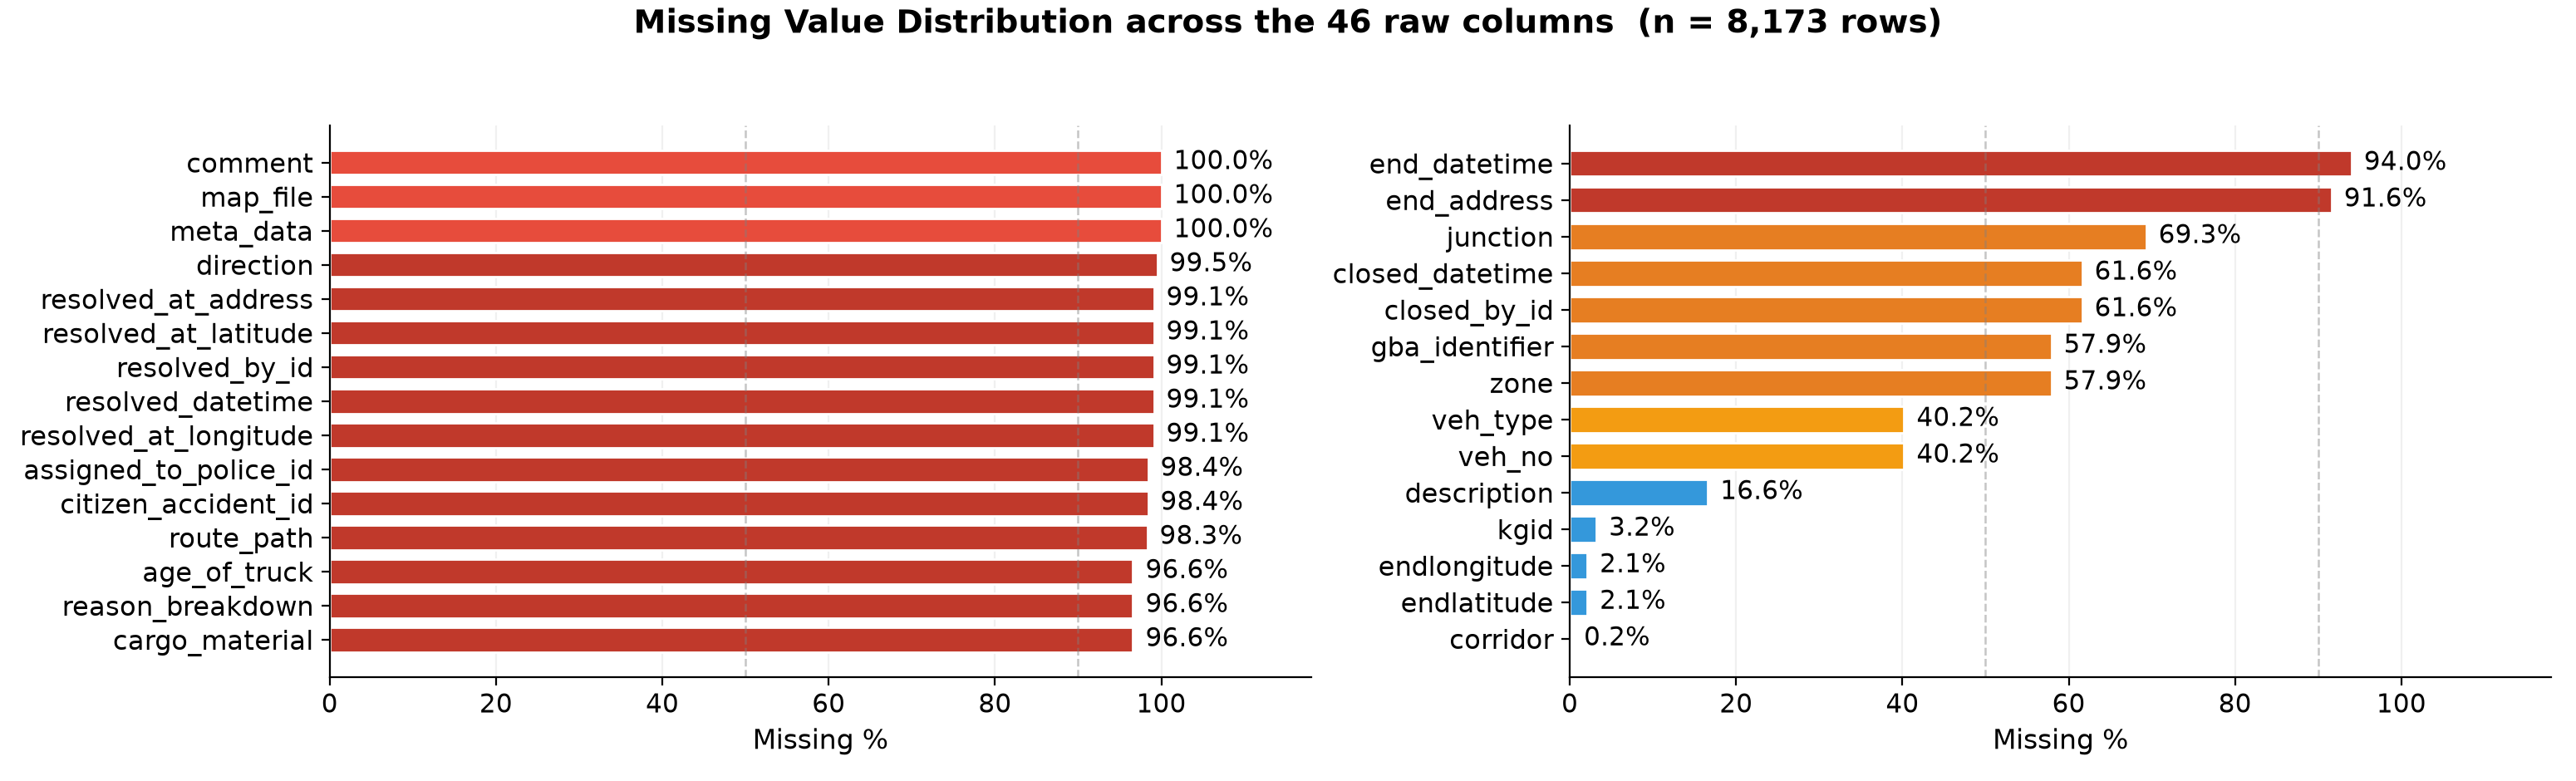
\includegraphics[width=0.95\textwidth]{figs/missing_values_wide.png}

  \vspace{2.5mm}
  \footnotesize
  \setlength{\tabcolsep}{5pt}
  \renewcommand{\arraystretch}{1.3}
  \begin{tabular}{>{\raggedright\arraybackslash}p{4.3cm}
                  >{\raggedright\arraybackslash}p{9.0cm}}
    \toprule
    Decision & Columns \\
    \midrule
    \bad{Dropped} \ (96--100\% missing) &
      \texttt{comment}, \texttt{map\_file}, \texttt{meta\_data}, resolution and
      truck fields \\
    \amb{Kept as ``unknown''} \ (40--70\%) &
      \texttt{junction}, \texttt{closed\_datetime}, \texttt{zone},
      \texttt{veh\_type} \\
    \good{Retained} \ (0\% missing) &
      coordinates, event cause, priority, closure flag \\
    \bad{Dropped} \ (identifiers) &
      \texttt{id}, \texttt{client\_id}, \texttt{created\_by\_id} \\
    \bottomrule
  \end{tabular}
\end{frame}
